\documentclass{article}

\usepackage[bib,bibstyle=ieee,bibargs={sorting=none},smalltitle,code,margin=0.95in]{shorthand}
\usepackage{pgfplots,pgfplotstable}
\usepackage{subfig}

\addbibresource{Report.bib}

\def\datafirst{2019-04-11-00-59-39}
\def\datasecond{2019-04-10-14-19-44}

\setcounter{secnumdepth}{0}

\title{Solving Differential Equations using a Forward Neural Network}
\author{Hunter Damron}
\date{11 April 2019}

\hdef{y}

\begin{document}
    \maketitle

    \section{Introduction}
        Although it originated as a mathematical model of neural activity, the forward neural network has become a popular tool in modern scientific culture. The neural network first gained popularity with Rosenblatt's perceptron~\cite{rosenblatt} and has since become widely used for function modeling with the increase in available computational power. Forward neural networks are composed of many `neurons' which are composed of a linear unit wrapped in a nonlinear function. Although the model is simple, it is capable of approximating any function, as shown by Cybenko~\cite{approx}.

    \section{Problem Statement}
        This paper presents for part 1 a simple neural network to approximate the function $y = \sin(kt)$ on the range $[0,2\pi/k]$ using points on the curve as training input. The resulting approximator is then generalized to the range $[0,k\pi]$. Part 2 uses a similar method to train a neural network to approximate a differential equation $y(t)$ given the constraints
        \begin{equation}\label{eqn:ode}
        \begin{gathered}
            y''(t) + k^2 y(t) = 0 \\
            y'(0) = 0.5 \\
            y(0) = 0
        \end{gathered}
        \end{equation}
        without any prior knowledge of the function. For both parts, a value of $k=10$ is used. For part 1, the network is trained against the network, but for part 2, the network is only compared against

    \section{Procedure}
        To effectively model the curve $y = \sin(kt)$, a neural network with two hidden layers of 120 nodes each is trained using mean square error ($MSE$). The input $t$ and output $\hy$ are both real scalars. Each layer other than the input layer is composed of a weight matrix $W_i \in \R^{n \times m}$ and a bias $b_i \in \R^m$ where $n$ is the input dimension and $m$ is the output dimension. Every layer except the last layer is also wrapped in an activation function $f_i$ to provide nonlinearity. Combining these pieces, each layer can be formulated as
        \begin{equation}
            x_{i+1} = f(W_i x_i + b_i)
        \end{equation}
        where $x_i$ is the input to the layer and $x_{i+1}$ is the layer's output. The choice of two layers with width 120 was found experimentally to be satisfactory for both approximations. For part 1, a Rectified Linear Unit ($ReLU = \max(0, x)$) was used as the activation function. For part 2, the $\tanh$ function was used instead because the differential equation constraints in Equation~\ref{eqn:ode} require a differentiable network.

        For training in part 1, the cost function was chosen to be the mean square error ($MSE$) of the predicted $\hy$ versus the true value $y$
        \begin{equation}
            J = MSE = \frac{1}{N} \sum_{i=0}^{N-1} (\hy(t_i) - y(t_i))^2
        \end{equation}
        where each $t_i$ is a sample point on the training range and $N$ is the number of samples. This cost function is a common choice for many machine learning applications because it is equivalent to the $L_2$-norm up to ordering but is more efficient and numerically stable because it does not take the square root. Although it is not necessary computationally, a batch method is used with each epoch consisting of 50 separate batches of 10 random samples. The batch method allows more rounds of training to be performed, often resulting in a better approximation. To help avoid local minima, the weight matrices $W_i$ are initialized element-wise with a random normal distribution. The biases $b_i$ are initialized at 0.

        Because for part 2 there is no known target function, the cost function used in part 1 is infeasible. Rather, the contraints in Equation~\ref{eqn:ode} were formulated into a cost function
        \begin{equation}
            J = \frac{1}{2N} \sum_{i=0}^{N-1} (y''(t_i) + k^2 y(t_i))^2 + (y'(0) - 0.5)^2 + y(0)^2
        \end{equation}
        which minimizes the residuals of each constraint. The factor of $1/2$ is included in the first term to emphasize the initial conditions but it does not affect the target function. This network is trained on the range $[0,k]$.

        The Adam algorithm presented in~\cite{adam} was used for optimization with a decaying learning rate. The Adam algorithm was chosen because it requires few parameters and is less susceptible to local minima because of its stochastic nature. The gradient descent algorithm was also able to provide good results but was found experimentally to be slower and more likely to fall into local minima than the Adam algorithm. A decaying learning rate was chosen to allow Adam to initially explore many possible approximations but allow it to become more precise after many epochs of training. For part 1, the initial learning rate was chosen to be 0.0005 while in part 2, and initial rate of 0.001 was used. Part 2 used a larger rate because the general structure of the target function was more complex. In both cases, the learning rate was set to decay by 0.95 every 1000 epochs.

        The TensorFlow framework~\cite{tf} was used for all numerical calculations in the project. A schematic of the network is shown in Figure~\ref{fig:network}. For part 2, the analytical solution to the differential equation is solved using the SymPy library~\cite{sympy}, allowing a programmatic comparison for any choice of $y(0)$ and $y'(0)$.

        \begin{figure}[!htbp]
            \centering
            \caption{Schematic of the network (produced using NN-SVG~\cite{schematic})} \label{fig:network}
            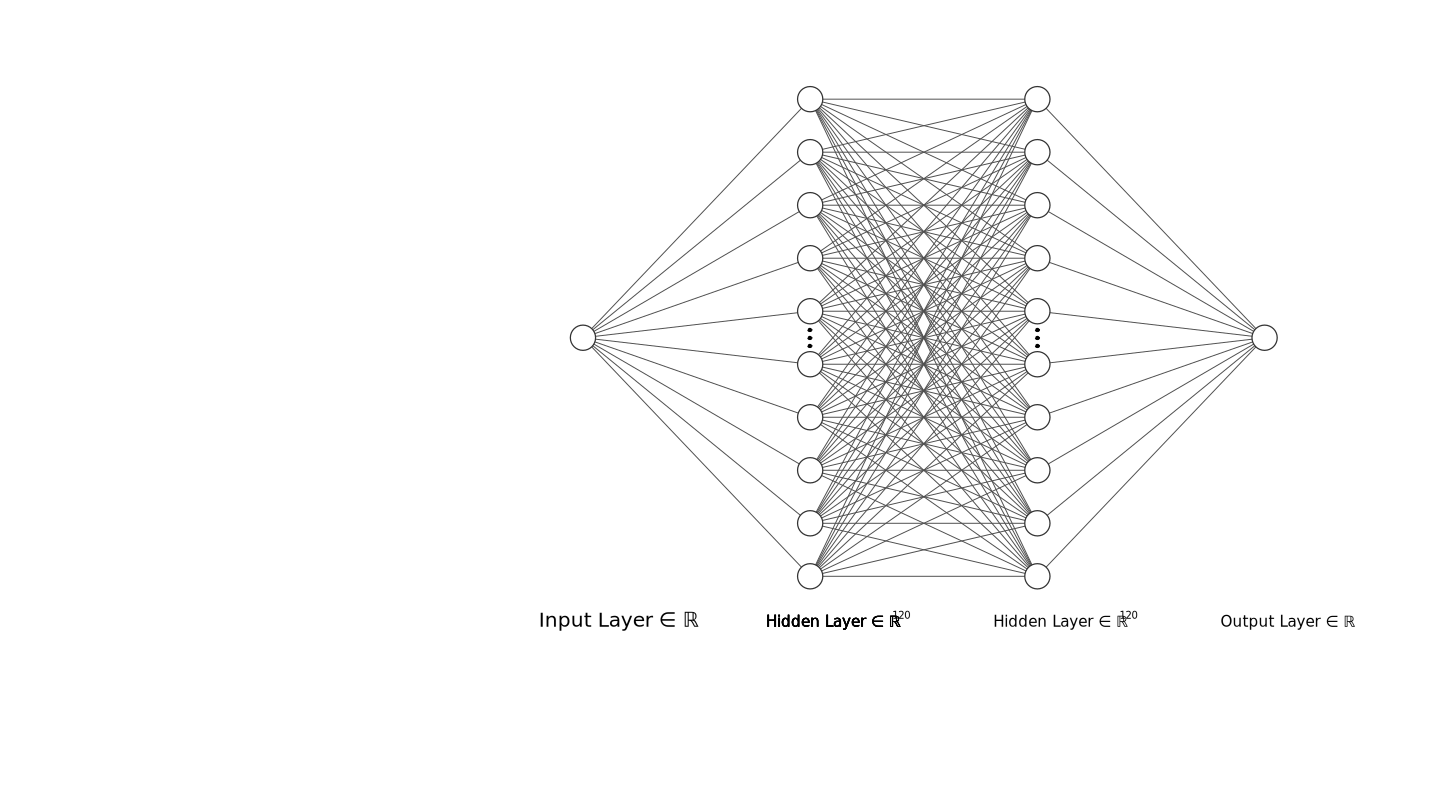
\includegraphics[width=0.8\textwidth]{nn.png}
        \end{figure}

    \section{Results}
        The results of the trained algorithm are shown in Figure~\ref{fig:output} as a comparison to the target $y=\sin(kt)$ on the training range $[0,2\pi/k]$. Figure~\ref{fig:full} shows the prediction of the network when extrapolated to a much larger range $[0,k\pi]$.

        \begin{figure}[!htbp]
            \centering
            \caption{Comparison of trained approximation $\hy$ to true value of $y$ on range $[0,2\pi/k]$} \label{fig:output}
            \begin{tikzpicture}
            \begin{axis}[
                    xlabel={$t$},
                    ylabel={$y$},
                    width=0.7\textwidth
                ]
                \pgfplotstableread[col sep=comma]{\datafirst/Values.csv}\datavalues
                \addlegendentry{Target}
                \addplot[thick,blue,mark=none,smooth,dashed] table[x index=0, y index=1]{\datavalues};

                \addlegendentry{Experimental}
                \addplot[thick,red,mark=none,smooth] table[x index=0, y index=2]{\datavalues};
            \end{axis}
            \end{tikzpicture}
        \end{figure}

        \begin{figure}[!htbp]
            \centering
            \caption{Comparison of trained approximation $\hy$ to true value $y$ when extrapolated to range $[0,k\pi]$} \label{fig:full}
            \begin{tikzpicture}
            \begin{axis}[
                    xlabel={$t$},
                    ylabel={$y$},
                    width=0.7\textwidth
                ]
                \pgfplotstableread[col sep=comma]{\datafirst/Values-full.csv}\datavaluesfull
                \addlegendentry{Target}
                \addplot[thick,blue,mark=none,smooth,dashed] table[x index=0, y index=1]{\datavaluesfull};

                \addlegendentry{Experimental}
                \addplot[thick,red,mark=none,smooth] table[x index=0, y index=2]{\datavaluesfull};
            \end{axis}
            \end{tikzpicture}
        \end{figure}

        Figure~\ref{fig:loss} shows the value of the loss function over time during training both on the training range and on the generalized range. Note that although the loss on the generalized range in Figure~\ref{fig:lossfull} decreases, it is quite large.

        \begin{figure}[!htbp]
            \centering
            \caption{Cost of $\hy$ versus $y=sin(kt)$ on training range and on generalized range}\label{fig:loss}
            \subfloat[On Range {$[0,2\pi/k]$}]{%
                \centering
                \begin{tikzpicture}
                \begin{axis}[
                	xlabel={Epoch},
                    ylabel={Cost $J$ (logarithmically scaled)},
                    ymode=log,
                    width=0.45\textwidth
               	]
                    \addplot[thick,mark=none,smooth] table[x expr={\coordindex}, y index=0,col sep=comma]{\datafirst/Losses.csv};
                \end{axis}
                \end{tikzpicture}
            }
            \hfill
            \subfloat[Generalized to range {$[0,k\pi]$} \label{fig:lossfull}]{%
                \centering
                \begin{tikzpicture}
                \begin{axis}[
                    xlabel={Epoch},
                    ylabel={Cost $J$ (logarithmically scaled)},
                    ymode=log,
                    width=0.45\textwidth
                ]
                    \addplot[thick,mark=none,smooth] table[x expr={\coordindex}, y index=1,col sep=comma]{\datafirst/Losses.csv};
                \end{axis}
                \end{tikzpicture}
            }
        \end{figure}

        Figure~\ref{fig:ode} plots the learned solution to the differential equation compared to the analytical solution $y=\frac{y'(0)}{k} \sin(kt)$. The loss of the learning process over each epoch is plotted in Figure~\ref{fig:odeloss}. Note that only every 10\textsuperscript{th} point is plotted in Figure~\ref{fig:odeloss}.

        \begin{figure}
            \centering
            \caption{Learned function approximating differential constraints in Equation~\ref{eqn:ode}}\label{fig:ode}
            \begin{tikzpicture}
                \begin{axis}[
                    xlabel={$t$},
                    ylabel={$y$},
                    width=0.7\textwidth
                ]

                    \addlegendentry{Target}
                    \addplot[thick,blue,mark=none,smooth,dashed] table[x index=0, y index=1, col sep=comma]{\datasecond/Values.csv};

                    \addlegendentry{Experimental}
                    \addplot[thick,red,mark=none,smooth] table[x index=0, y index=2, col sep=comma]{\datasecond/Values.csv};
                \end{axis}
            \end{tikzpicture}
        \end{figure}

        \begin{figure}
            \centering
            \caption{Cost function of learning instance in shown in Figure~\ref{fig:ode}}\label{fig:odeloss}
            \begin{tikzpicture}
                \begin{axis}[
                    xlabel={Epoch},
                    ylabel={Cost $J$ (logarithmically scaled)},
                    ymode=log,
                    width=0.7\textwidth
                ]
                     \addplot[thick,mark=none,smooth] table[x expr={\coordindex*10}, y index=1, col sep=comma]{\datasecond/Losses-trimmed.csv};
                \end{axis}
            \end{tikzpicture}
        \end{figure}

    \section{Discussion}
        In part 1, training on the range $[0,2\pi/k]$ was achieved on the order of minutes using the described configuration and produced a decent result. With a more precise tuning of the parameters and possibly wider hidden layers, a neural network should be capable of easily approximating a single variable function on such a small range. However, when the range is extended to $[0,k\pi]$, the result is not accurate at all. After the training range, the network responds approximately linearly because there was no reason for it to change its behavior outside the training range. Although neural networks may be capable of interpolating missing data within the training range, it is nearly impossible for them to accurately extrapolate far beyond the training range.

        The loss function, as shown in Figure~\ref{fig:loss}, shows that the initial training happens very quickly, but the majority of training applies to the last small deviation. Attempts have been made in other optimizers to increase training speed on small deviations without sacrificing accuracy. In future exploration, these other optimization algorithms may be used. This rate of learning is also controlled by a hyperparameter which may not be optimally tuned.

        The learned approximation in part 2 differs significantly from the analytical solution, but it conforms to the constraints in Equation~\ref{eqn:ode} moderately well. The initial conditions are adequately learned, but the amplitude of the approximation is not constant like the target function. However, because the amplitude is dependent on the initial condition $y'(0)$, the decaying behavior results from the buildup of small deviations in the approximation which accumulate farther from $t=0$. With a much longer training time and more rapidly decaying learning rate, the approximation may have been able to achieve a more stable oscillation.
    \printbibliography{}

    \appendix
    \section{Appendix}
    \setcounter{secnumdepth}{2}
    \renewcommand{\thesubsection}{\Alph{subsection}}
    \subsection{Network Implementation} \label{apx:code}
    \lstinputlisting{DiffEq.py}
\end{document}
